\chapter{Especificación del diseño}\label{chap:design}

\section{Visión general}

Este capítulo tiene como objetivo describir la labor de diseño realizada para desarrollar el proyecto, así como las herramientas que han sido necesarias para su realización. En el siguiente listado se describen los aspectos de diseño que se van a explicar en este capítulo:

\begin{itemize}
	\item \textbf{Diseño de la aplicación cliente}: descripción de las modificaciones realizadas sobre una plantilla \acrshort{uwp}.
	\item \textbf{Diseño de la aplicación web}: descripcion de las modificaciones realizadas sobre una plantilla ASP.NET \acrshort{mvc}.

\end{itemize}

\section{Diseño de la aplicación cliente}

La Aplicación cliente cuenta con dos clases especiales para ocuparse de la lógica de las peticiones HTTP y de la lógica de uso de una cámara web.

\begin{figure}[!htbp]
	\centering
	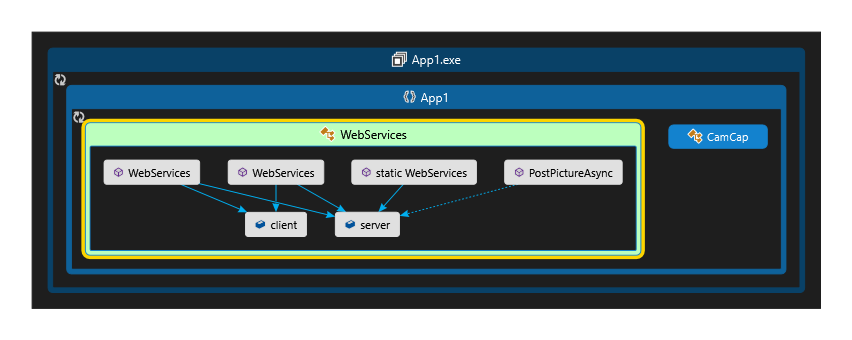
\includegraphics[angle=90, scale=1.0]{fig/WebServices}
	\caption{Clase WebServices}
\end{figure}

\FloatBarrier

\lstinputlisting[frame=single, caption=clase WebServices]{content/code/webservices.cs}

\begin{figure}[!htbp]
	\centering
	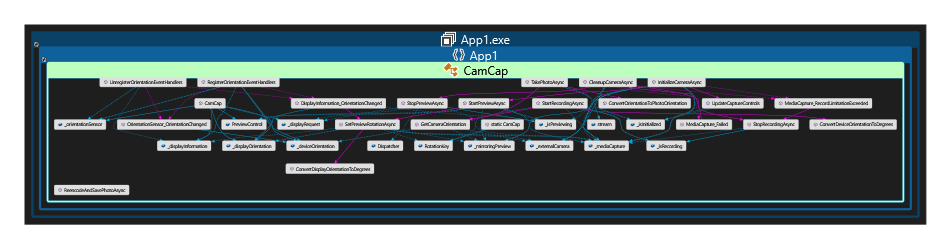
\includegraphics[angle=90, scale=0.9]{fig/CamCap}
	\caption{Clase CamCap}
\end{figure}

\FloatBarrier

Ya que la clase CamCap es en su mayoría parte de un ejemplo de Microsoft sobre el manejo correcto de una WebCam mediante la librería MediaCapture y no un código creado expresamente con el solo fin de capturar imágenes, la mayoría de los métodos, propiedades y variables del diagrama no se usan, aquí se incluyen las partes del código que se usan en el proyecto:

\begin{itemize}

\item \textbf{InitializeCameraAsync:} inicialización de la cámara.

\lstinputlisting[frame=single, caption=código de InitializeCameraAsync]{content/code/initializecamera.cs}

\item \textbf{StartPreviewAsync:} acceso a una vista previa de lo que será capturado por la cámara.

\lstinputlisting[frame=single, caption=código de StartPreviewAsync]{content/code/startpreview.cs}

\item \textbf{TakePhotoAsync:} se captura una imagen y se codifica en un stream.

\lstinputlisting[frame=single, caption=código de TakePhotoAsync]{content/code/takephoto.cs}

\end{itemize}

\section{Diseño de la aplicación web}

La principal inclusión en la plantilla de la aplicación Web es un controlador para abordar todas las funciones necesarias.

\begin{figure}[!htbp]
	\centering
	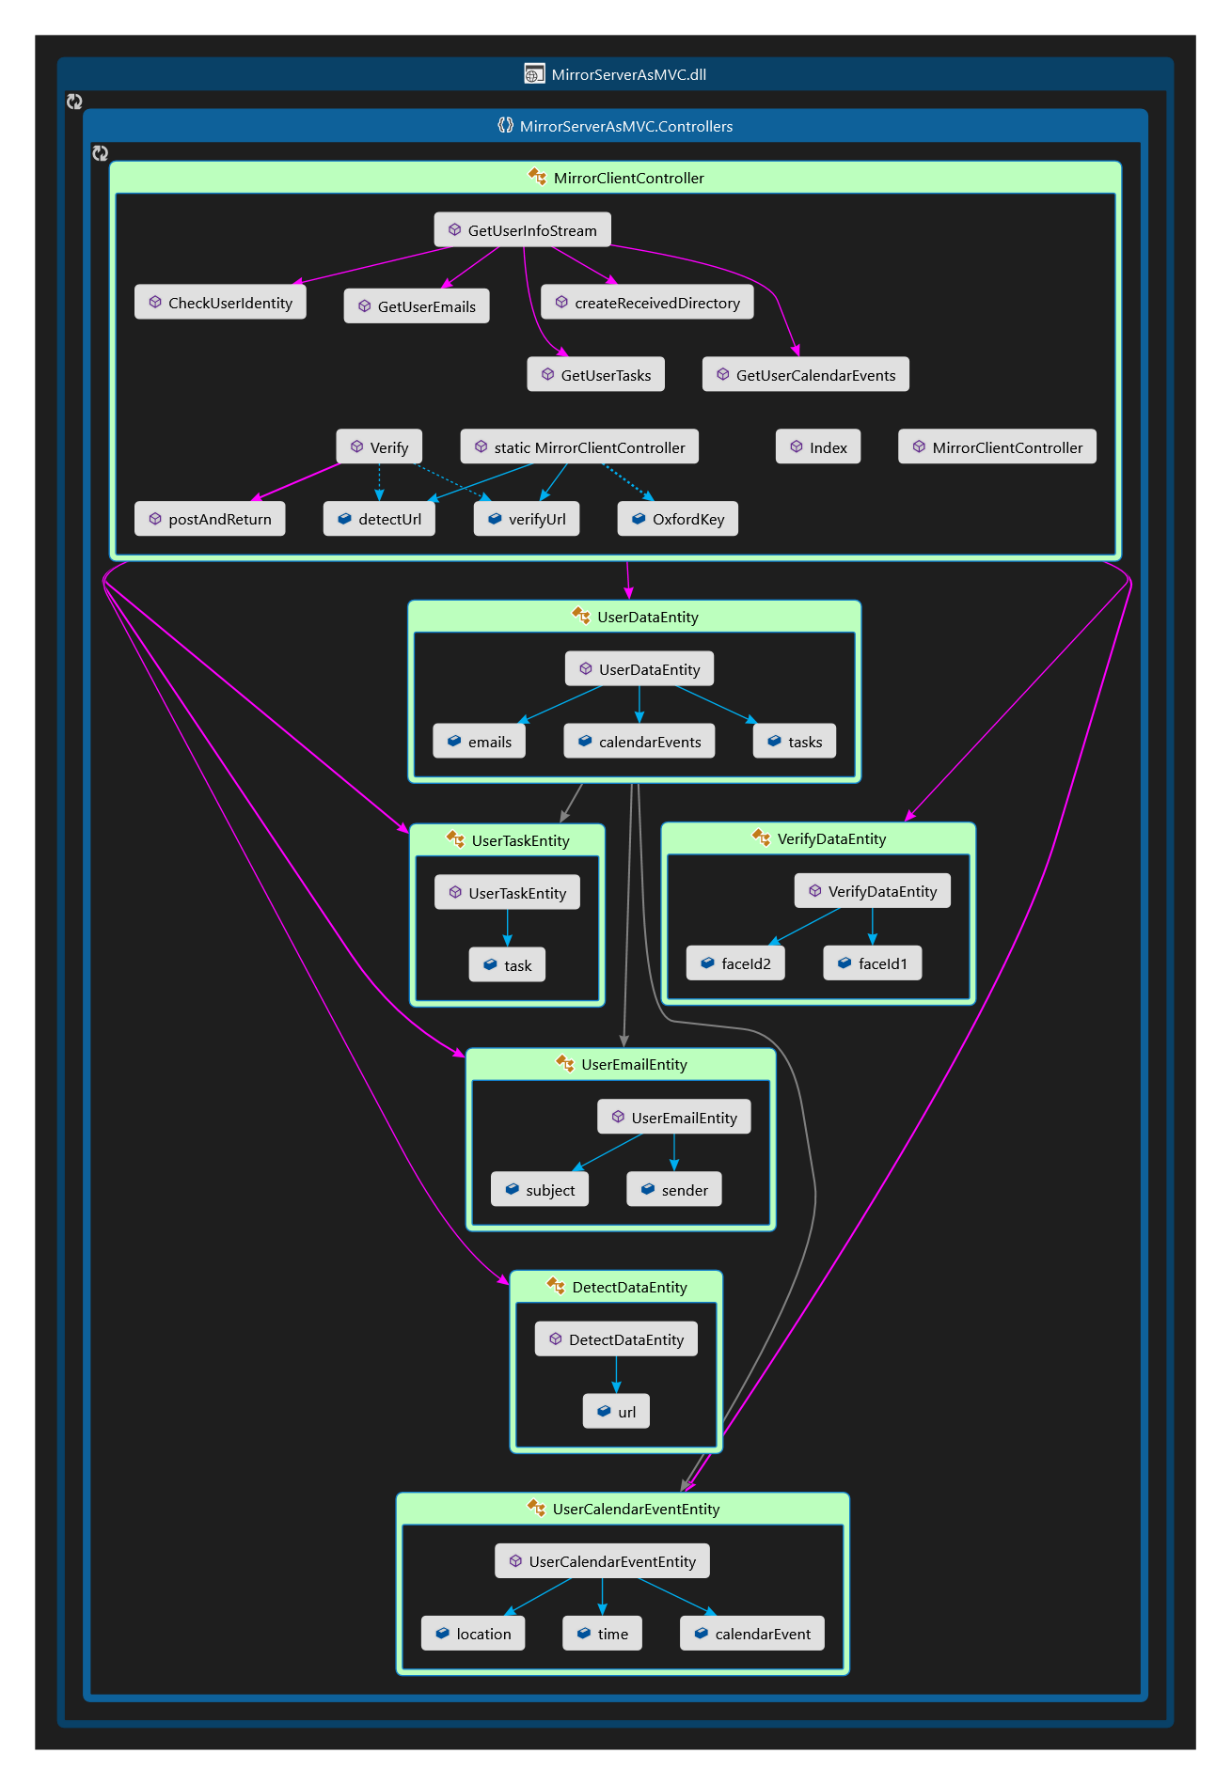
\includegraphics[angle=0, scale=1.0]{fig/MirrorClientController}
	\caption{Clase MirrorClientController}
\end{figure}

\FloatBarrier

A continuación se muestra el código que usa el servidor para recibir una imagen, almacenarla y usarla para verificar un usuario.

\lstinputlisting[frame=single, caption=fragmento de código de MirrorClientController]{content/code/controller.cs}

\subsection{Modificación de la \acrshort{bd}}

Una aplicación ASP.NET \acrshort{mvc} configurada con autenticación crea por defecto una \acrshort{bd} con todas las tablas necesarias para autenticar usuarios y usar roles, en el caso de este proyecto se modificó el esquema para incluir tres campos en la tabla del usuario:

\begin{itemize}
\item \textbf{FaceId:} un id de cara proporcionado por Microsoft Cognitive Services, que expira a las 24 horas de ser generado.
\item \textbf{LastUpdate:} fecha en la que se actualizó el identificador de cara por ultima vez para comprobar si está expirado o no.
\item \textbf{PhotoUrl:} URL a una imagen del usuario para obtener nuevos FaceId y contrastarlos con los de las fotos que se reciban desde el Smart Mirror.
\end{itemize}

\begin{figure}[!htp]
	\centering
	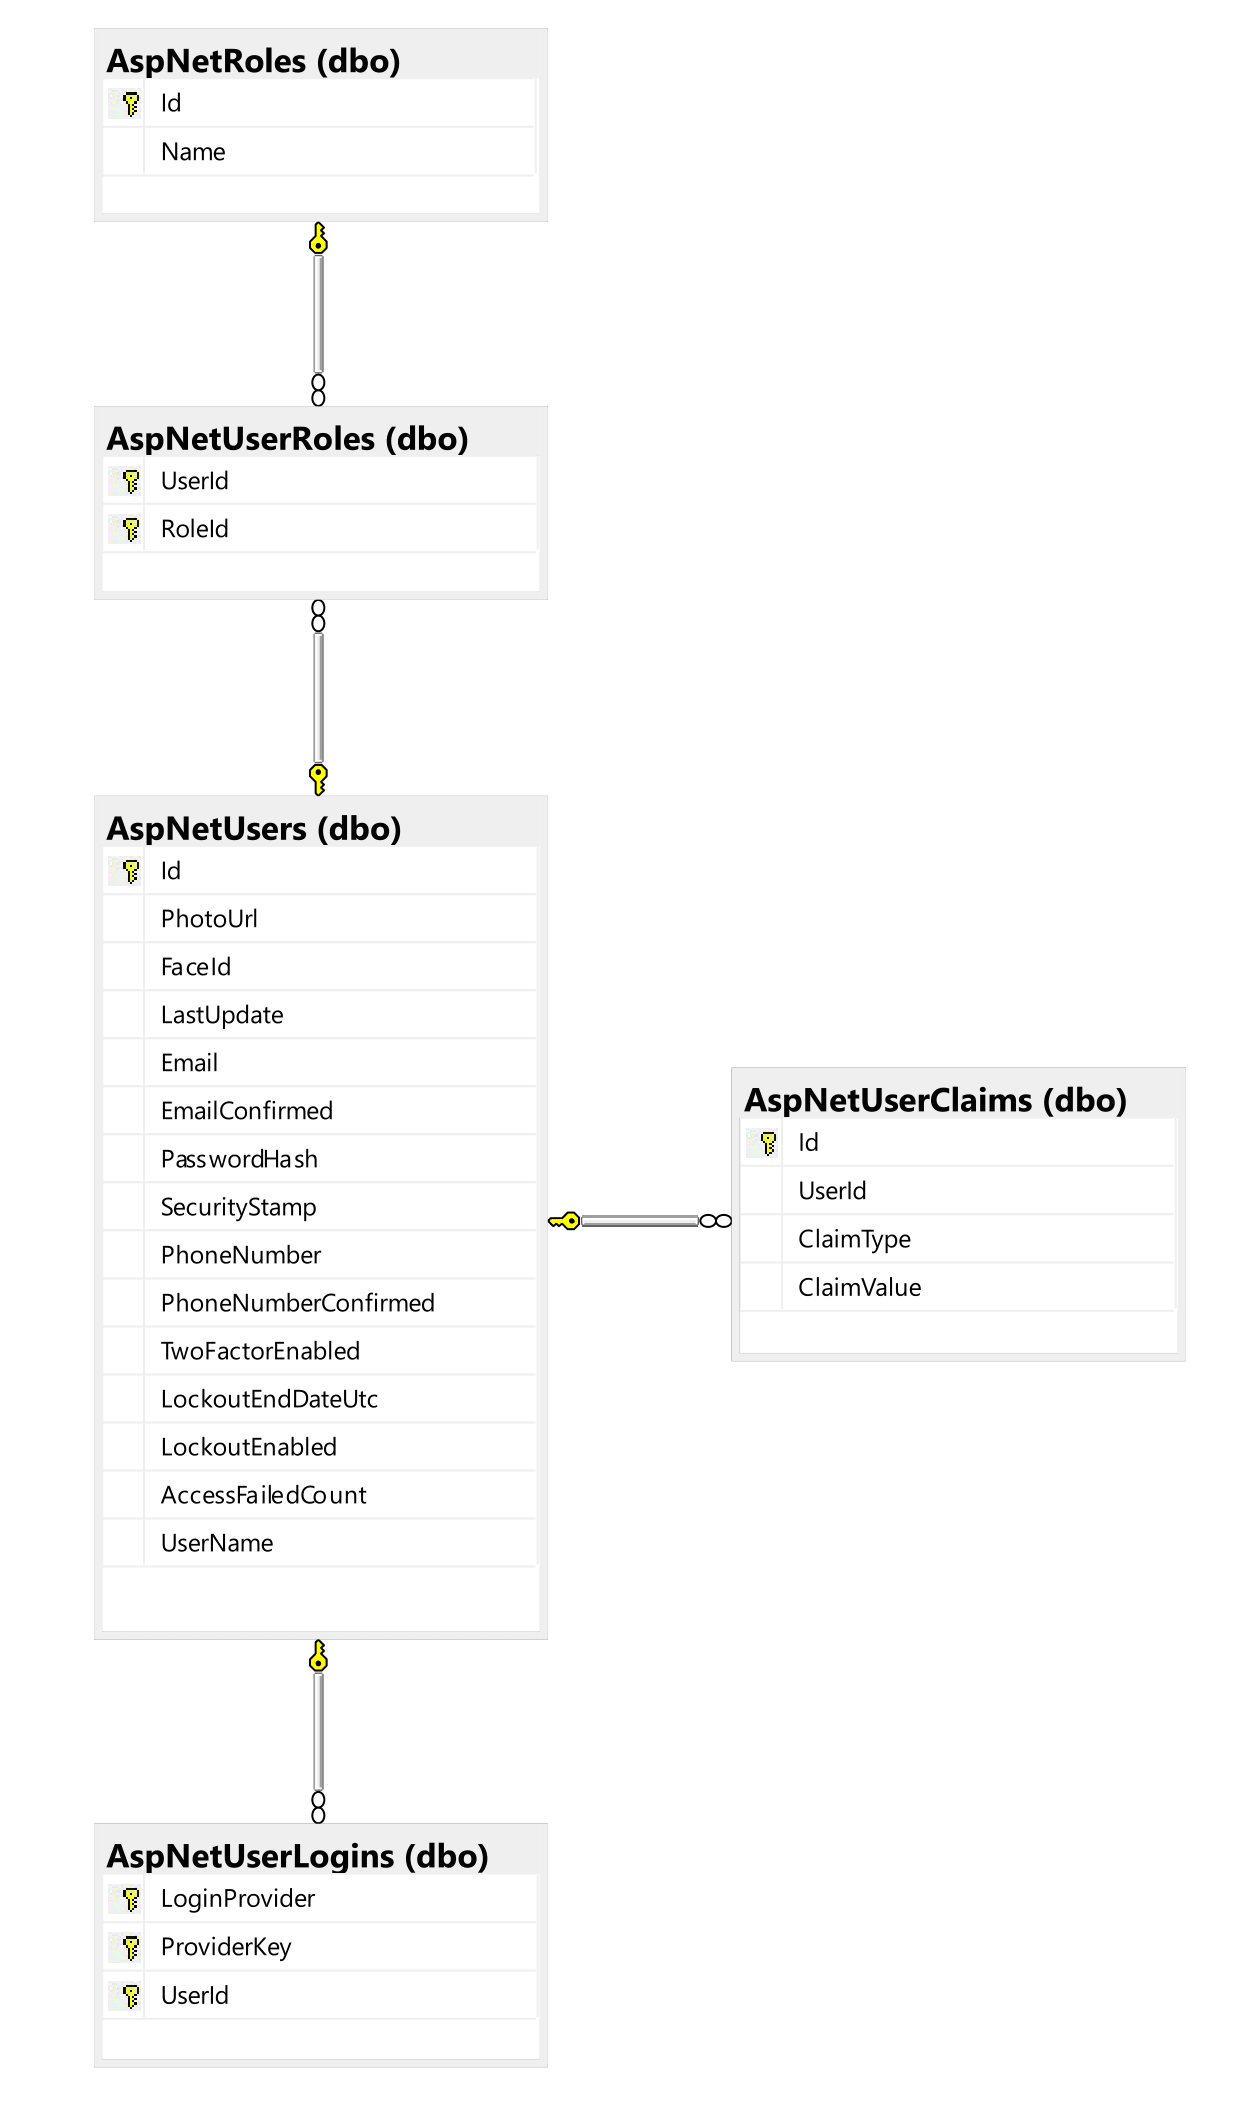
\includegraphics[angle=0, page=1, scale=.3]{fig/schema}
	\caption{Schema de la \acrshort{bd} modificada}
\end{figure}

\FloatBarrier
